\documentclass{llncs}
\usepackage{hyperref}
\usepackage{url}
\pagestyle{plain}
\usepackage{threeparttable}
\input{math_commands.tex}
%\usepackage[latin9]{inputenc}
%\usepackage[T1]{fontenc}
\usepackage{float}
\usepackage{wrapfig}
\usepackage{lineno}
\usepackage{amsmath}
\usepackage{amssymb}
\usepackage{graphicx}
\usepackage{subcaption}
\usepackage{tabularx}
\usepackage{cases}
\captionsetup{compatibility=false}
% \usepackage{esint}
\usepackage{array}
\usepackage{epstopdf}
\usepackage{placeins}
\usepackage{pgfplots}
\usepackage{url}
\usepackage{tikz}
\usepackage{calc}
\usepackage{array}
\usepackage[linesnumbered,ruled,vlined]{algorithm2e}
\usetikzlibrary{positioning, arrows.meta,calc}

%%%%%%%%%%%%%%%%%%%%%%%%%%%%%%%
%%%%%%%%%%%%%%%%%%%%%%%%%%%%%%%

\newcommand{\vW}{\boldsymbol{W}}
\newcommand{\val}{{\textrm{value}}}
\newcommand{\Val}{{\textrm{value}}}
\newcommand{\MILP}{{\textrm{MILP}}}
\newcommand{\LP}{{\textrm{LP}}}
\newcommand{\Improve}{\mathrm{Improve}}
\newcommand{\Utility}{\mathrm{SAS}}
\newcommand{\Sol}{\mathrm{Sol}}
\newcommand{\sol}{\mathrm{sol}}
\newcommand{\UB}{\mathrm{UB}}
\newcommand{\LB}{\mathrm{LB}}
\newcommand{\ub}{\mathrm{ub}}
\newcommand{\lb}{\mathrm{lb}}
\newcommand{\B}{\mathrm{B}}
\usepackage{amsmath, amssymb, amsfonts}
\newcommand{\ReLU}{\mathrm{ReLU}}
\newcommand{\CMP}{{\textrm{CMP}}\ }
\newcommand{\fix}{\marginpar{FIX}}
\newcommand{\new}{\marginpar{NEW}}
\newcommand{\toolname}{Hybrid MILP}


\title{Global case}
\date{}


\begin{document}
	
	\maketitle
	\linenumbers
	\begin{abstract}
		TODO
	\end{abstract}
	
	\section{Introduction}
	
	\section{Notations and Preliminaries}
	
	In this paper, we will use lower case latin $a$ for scalars, bold $\boldsymbol{z}$ for vectors, 
	capitalized bold $\boldsymbol{W}$ for matrices, similar to notations in \cite{crown}.
	To simplify the notations, we restrict the presentation to feed-forward, 
	fully connected ReLU Deep Neural Networks (DNN for short), where the activation function is $\ReLU : \mathbb{R} \rightarrow \mathbb{R}$ with
	$\ReLU(x)=x$ for $x \geq 0$ and $\ReLU(x)=0$ for $x \leq 0$, which we extend componentwise on vectors.
	
	%In this paper, we will not use tensors with a dimension higher than matrices: those will be flattened.
	
	%\subsection{Neural Network and Verification}
	
	
	% testtesttesttest
	An $\ell$-layer DNN is provided by $\ell$ weight matrices 
	$\boldsymbol{W}^i \in \mathbb{R}^{d_i\times d_{i-1}}$
	and $\ell$ bias vectors $\vb^i \in \mathbb{R}^{d_i}$, for $i=1, \ldots, \ell$.
	We call $d_i$ the number of neurons of hidden layer $i \in \{1, \ldots, \ell-1\}$,
	$d_0$ the input dimension, and $d_\ell$ the output dimension.
	
	Given an input vector $\boldsymbol{z}^0 \in \mathbb{R}^{d_0}$, 
	denoting $\hat{\boldsymbol{z}}^{0}={\boldsymbol{z}}^0$, we define inductively the value vectors $\boldsymbol{z}^i,\hat{\vz}^i$ at layer $1 \leq i \leq \ell$ with
	\begin{align*}
		\boldsymbol{z}^{i} = \boldsymbol{W}^i\cdot \hat{\boldsymbol{z}}^{i-1}+ \vb^i \qquad \, \qquad
		\hat{\boldsymbol{z}}^{i} = \ReLU({\boldsymbol{z}}^i).
	\end{align*} 
	
	The vector $\hat{\boldsymbol{z}}$ is called post-activation values, 
	$\boldsymbol{z}$ is called pre-activation values, 
	and $\boldsymbol{z}^{i}_j$ is used to call the $j$-th neuron in the $i$-th layer. 
	For $\boldsymbol{x}=\vz^0$ the (vector of) input, we denote by $f(\boldsymbol{x})=\vz^\ell$ the output. Finally, pre- and post-activation neurons are called \emph{nodes}, and when we refer to a specific node/neuron, we use $a,b,c,d,n$ to denote them, and $W_{a,b} \in \mathbb{R}$ to denote the weight from neuron $a$ to $b$. Similarly, for input $\boldsymbol{x}$, we denote by $\val_{\boldsymbol{x}}(a)$ the value of neuron $a$ when the input is $\boldsymbol{x}$.	For convenience, we write $n < z$ if neuron $n$ is on a layer before $\ell_z$, and $n \leq z$ if $n< z$ or $n=z$.
	
	Concerning the verification problem, we focus on the global-robustness question. Global robustness asks to determine how the output of a neural network will be affected under a certain kind of small perturbations to any possible input. In this view, Lipschitz continuity is a good characterization of global robustness.
	
	
	
	
	\section{Global robustness and Lipschitz constant}
	
	
	Recall the definition of Lipschitz continuity:
	under distance $d$, a function $f(x)$ is Lipschitz continuous with respect to constant $K$ if:
	\begin{align*}
		\forall \boldsymbol{x} \forall\boldsymbol{y} (|f(\boldsymbol{x}) -f(\boldsymbol{y}) |\leq K|\boldsymbol{x}-\boldsymbol{y}|)
	\end{align*} 
	In our practice, when we need global robustness, we will compute an optimization question respect to a certain number $\varepsilon$:	\begin{align}\label{global_robustness}
		\max_{|\boldsymbol{x}-\boldsymbol{y}| \leq \varepsilon} |f(\boldsymbol{x}) -f(\boldsymbol{y}) |
	\end{align} And this will lead to the following definition

		\begin{definition}[$\varepsilon$-diff bound]
		Suppose we have a function $f$ from $\mathbb{R}^n$ to $\mathbb{R}^m$ and $||$ is $L_\infty$ norm. 
		
		For a number $\varepsilon\in\mathbb{R}$, an $\varepsilon$-diff bound $D_\varepsilon$ is a number such that for any inputs $x,y$: \begin{align*}
			|x-y|\leq \varepsilon \implies |f(x)-f(y)| \leq D_\varepsilon \cdot \varepsilon
		\end{align*}
		
	\end{definition}
	
	From $\varepsilon$-diff bound, we cannot directly obtain a Lipschitz bound for the function, but we can get the following weaker bound:
	
	\begin{definition}[Lipschitz above $\varepsilon$ constant]
		Suppose we have a function $f$ from $\mathbb{R}^n$ to $\mathbb{R}^m$ and $||$ is $L_\infty$ norm. 
		
		For a number $\varepsilon\in\mathbb{R}$, a Lipschitz above $\varepsilon$ constant  $K_\varepsilon$,  is a number such that for any inputs $x,y$: \begin{align*}
			|x-y|\geq \varepsilon &\implies |f(x)-f(y)| \leq K_\varepsilon \cdot |x-y|\\
			|x-y|<\varepsilon &\implies |f(x)-f(y)| \leq K_\varepsilon \cdot \varepsilon\\
		\end{align*}
		
	\end{definition}
	
	
	\begin{proposition}
		
		Suppose $D$ is an $\varepsilon$-diff bound for $f(x)$. Then for any $N\in\mathbb{Z}^+$, $D\frac{N+1}{N}$ is a Lipschitz about $N\varepsilon$ constant.
		
		That is, for any two inputs $x,y$, if \begin{align*}
			|x-y|\leq \varepsilon \implies |f(x)-f(y)| \leq D \cdot \varepsilon,
		\end{align*} then 	 \begin{align*}
			|x-y|\geq N\varepsilon &\implies |f(x)-f(y)| \leq D\frac{N+1}{N} \cdot |x-y|\\
			|x-y|<N\varepsilon &\implies |f(x)-f(y)| \leq D\frac{N+1}{N} \cdot N\varepsilon\\
		\end{align*}
	\end{proposition}
	
	\begin{proof} We fix the number $N\in\mathbb{Z}^+$ and assume we have two inputs $x, y$.
		
		The first case, $|x-y|\geq N\varepsilon$. Then we assume $|x-y| \in [M\varepsilon ,  (M+1)\varepsilon]$ for another integer $M\geq N$. Then we can divide the line segment between $x, y$ into $M+1$ pieces: $x_0 = x, x_1, x_2, \cdots, x_{M+1} = y$ such that $|x_i-x_{i+1}| \leq \varepsilon$ and apply the definition of $\varepsilon$-diff bound $D$ for each pieces:\begin{align*}
			|f(x)-f(y)| &= |f(x_{M+1})-f(x_M)+\cdots+f(x_1)-f(x_0)|\\
			&\leq |f(x_{M+1})-f(x_M)|+\cdots+|f(x_1)-f(x_0)|\\
			&\leq D\varepsilon + \cdots +D\varepsilon = (M+1)D\varepsilon
		\end{align*}
		Hence,\begin{align*}
			|f(x)-f(y)| &\leq (M+1)D\varepsilon \leq D\cdot (M+1)\varepsilon \frac{|x-y|}{M\varepsilon}\\
			&= D\cdot\frac{M+1}{M} |x-y|	\leq   D\cdot\frac{N+1}{N} |x-y|		
		\end{align*}
		The second case, $|x-y|< N\varepsilon$. Similarly we can divide the line segment between $x, y$ into $N$ pieces and then $|f(x)-f(y)|\leq D N\varepsilon\leq |f(x)-f(y)|\leq D \frac{N+1}{N} N\varepsilon$.
		
		This ends the proof.
	\end{proof}

	In practice, Lipschitz above $\varepsilon$ constant is already sufficient, since in most cases we care about the absolute difference under input perturbations, not the ratio. By combining the above proposition, the computation of $\varepsilon$-diff bound can satisfy our aim.
	

	Moreover, we have one more proposition connecting $\varepsilon$-diff bound and Lipschitz above $\varepsilon$ constant.
	
	
	\begin{proposition}
		For any $N\in\mathbb{Z}^+$, suppose for any $a$ in $\{\frac{N}{N}\varepsilon,\frac{N+1}{N}\varepsilon,\cdots, \frac{2N-1}{N}\varepsilon\}$, $D$ is an $a$-diff bound for $f(x)$. 
		
		Then $D\frac{N+1}{N}$ is a Lipschitz about $\varepsilon$ constant:\begin{align*}
			|x-y|\geq \varepsilon &\implies |f(x)-f(y)| \leq D\frac{N+1}{N} \cdot |x-y|\\
			|x-y|<\varepsilon &\implies |f(x)-f(y)| \leq D\frac{N+1}{N} \cdot \varepsilon\\
		\end{align*}
	\end{proposition}
	\begin{proof}
		We fix the number $N\in\mathbb{Z}^+$ and assume we have two inputs $x, y$.
		
		For the case that $|x-y|<\varepsilon$, this is trivial by definition.
		
		For the case that $|x-y|\geq \varepsilon$, there exists a sum $x_1+x_2+\cdots+x_n$ by numbers from (allowing repetitions) $\{\frac{N}{N}\varepsilon,\frac{N+1}{N}\varepsilon,\cdots, \frac{2N-1}{N}\varepsilon\}$ such that \begin{align*}
			\varepsilon \leq x_1+x_2+\cdots+x_n -\frac{1}{N}\varepsilon \leq |x-y| \leq x_1+x_2+\cdots+x_n
		\end{align*}
		By assumption, divide the line segment from $x$ to $y$ into pieces according to $x_1, x_2,\cdots,x_n$, then we will have $$|f(x)-f(y)|\leq Dx_1+Dx_2+\cdots+Dx_n.$$
		
			Hence,\begin{align*}
			\dfrac{|f(x)-f(y)|}{|x-y|} &\leq \dfrac{Dx_1+Dx_2+\cdots+Dx_n}{x_1+x_2+\cdots+x_n -\frac{1}{N}\varepsilon}\\
			& \leq D\cdot( 1+  \dfrac{\frac{1}{N}\varepsilon}{\varepsilon})= D \frac{N+1}{N}\\
		\end{align*}
		This ends the proof.
	\end{proof}
	
	
	
	\section{pMILP for local robustness}
	
	
	
	\subsection{MILP and LP encodings for DNNs}
	
	First we introduce some concepts for local robustness question.
	
	Mixed Integer Linear Programming (MILP) value abstraction is a complete (but inefficient) method. 
	For an unstable neuron $n$ that its value $x \in [\LB(n),\UB(n)]$ with $\LB(n)<0<\UB(n)$, the value $\hat{x}$ of $\ReLU(x)$ can be encoded exactly in an MILP formula with one 
	integer variable $a$ valued in $\{0,1\}$, using constants $\UB(n),\LB(n)$ with 4 constraints \cite{MILP}:
	
	\vspace{-0.4cm}
	\begin{equation}\quad \hat{x} \geq x \quad \wedge \quad \hat{x} \geq 0, \quad \wedge \quad \hat{x} \leq \UB(n) \cdot a \quad \wedge \quad \hat{x} \leq x-\LB(n) \cdot (1-a)
		\label{eq11}
	\end{equation}
	
	%For all $x \in [\LB(n),\UB(n)] \setminus 0$, there exists a unique solution $(a,\hat{x})$ that meets these constraints, with $\hat{x}=\ReLU(x)$ \cite{MILP}. The value of $a$ is 0 if $x < 0$, and 1 if $x>0$, and can be either if $x=0$. This encoding approach can be applied to every (unstable) ReLU node, and optimizing its value can help getting more accurate bounds. However, for networks with hundreds of {\em unstable} nodes, the resulting MILP formulation will contain numerous integer variables and generally bounds obtained will not be accurate, even using powerful commercial solvers such as Gurobi.
	
	The global structure is as follows, using Gurobi as an example:
	\begin{enumerate}
		\item For each input node, each output node, and each pre-activation and post-activation node in the hidden layers,  set one variable. 
		\item Set constraints for input nodes.
		\item For each pre-activation node in a hidden layer (and each output node), set linear constraints relating them to the post-activation or input nodes in the previous layer they connect to.
		\item Between pre- and post- activation nodes, set the MILP constraint described above.
	\end{enumerate} We use $\mathcal{M}$ to denote the whole MILP model. In practice, we may only consider the network up to a certain hidden layer. In that case, the pre-activation nodes of that layer serve as the output nodes of the model $\mathcal{M}$.
	
	MILP instances can be linearly relaxed into LP over-abstraction, where variables originally restricted to integers in $\{0,1\}$ (binary) are relaxed to real numbers in the interval $[0,1]$, while maintaining the same encoding. As solving LP instances is polynomial time, this optimization is significantly more efficient. However, this efficiency comes at the cost of precision, often resulting in less stringent bounds. This approach is termed the {\em LP abstraction}. We invoke a folklore result on the LP relaxation of (\ref{eq11}), for which we provide a direct and explicit proof.
	
	
	\subsection{partial MILP}
	
	We will use {\em partial MILP} (pMILP for short, see \cite{DivideAndSlide}) to get trade-offs between accuracy and runtime. Here, we extract the explanation from paper CITE.
	
	
	Let $X$ be a subset of the set of unstable neurons, and $n$ a neuron for which we want to compute upper and lower bounds on values: the partial MILP based on $X$ to compute neuron $n$ simply calls Gurobi to minimize/maximize the value of $n$ with the MILP model encoding, where variable $a$ is:
	\begin{itemize}
		\item binary for neurons in $X$ (exact encoding of the ReLU),
		\item linear for neurons not in $X$ (linear relaxation).
	\end{itemize}
	We will denote above case by MILP$_X$ or $\mathcal{M}_X$. Informally, we say that a node is opened if it is in $X$. 
	
	If $X$ covers all unstable neurons, then MILP$_X$ is exact. But then the time cost may be very large (exponential growth).
	
	
	To reduce the runtime, we will limit the size of subset $X$. This a priori hurts accuracy. To recover some of this accuracy, we use an iterative approach: computing lower and upper bounds $\LB,\UB$ for neurons $n$ of a each layer iteratively, that are used when computing values of the next layer.
	
	
	\subsection{SAS}
	
	
	In pMILP, to decide the set $X$, we introduce the method {\em Solution-Aware Scoring} (SAS)
	to evaluate accurately how opening a ReLU impacts the accuracy. Again, here we use the definition from paper CITE. For details and explanation, see CITE.
	
	
	Assume that we want to compute an upper bound for neuron $z$ on layer $\ell_z$. For each node $n<z$, we denote ($\Sol\_\max_X^z(n))_{n \leq z}$ a solution of $\mathcal{M}_X$ maximizing $z$: $\Sol\_\max_X^z(z)$ is the maximum of $z$ under $\mathcal{M}_X$; and we denote $(\sol(n))_{n \leq z} = (\Sol\_\max_\emptyset^z(n))_{n \leq z}$ a solution maximizing the value for $z$ when all ReLU use the LP relaxation. Moreover,  we define the function
	$\Improve\_\max^z(n)=$ $\sol(z) - \Sol\_\max_{\{n\}}^z(z)$, 
	accurately represents how much opening neuron $n < z$ reduces the maximum computed for $z$
	compared with using only LP. 
	
	First, SAS will call solvers to compute the LP model to get a solution, which is reasonably fast as there is no binary variables. 
	
	Next, for a neuron $b$ on the layer before layer $\ell_z$, we define:
	
	
	\vspace{-0.4cm}
	$$\Utility\_\max\nolimits^z(b) = W_{bz} \times (\sol(\hat{b})- \ReLU(\sol(b)))$$
	\vspace{-0.4cm}
	
	
	And for a neuron $a$ two layers before $\ell_z$, 
	$b$ denoting neurons in the layer $\ell$ just before $\ell_z$.
	Recall the rate $r(b)=\frac{\max(0,\UB(b))}{\max(0,\UB(b))-\min(0,\LB(b))} \in [0,1]$.
	We define:
	
	
	\begin{flalign*}
		\Delta(\hat{a}) &= \ReLU(\sol(a))-\sol(\hat{a})&&\\
		\forall b \in \ell, \Delta(b) &= W_{ab}\Delta(\hat{a})&&\\	
	\end{flalign*}
	
	\vspace{-1.2cm}
	
	\begin{subnumcases}{\forall b \in \ell, \Delta(\hat{b}) =}
		r(b)\Delta(b), & for $W_{bz} > 0$ \\
		\max(\Delta(b),-\sol(b)), & for $W_{bz} < 0$ and $\sol(b)\geq0$\\
		\max(0,\Delta(b)+\sol(b)), & for $W_{bz} < 0$ and $\sol(b)<0$ \quad \, \quad \, \quad		 
	\end{subnumcases}
	
	\begin{flalign*}
		\Utility\_\max\nolimits^z(a) &= \Delta(z) = -\sum_{b \in \ell} W_{bz} \Delta(\hat{b})&&
	\end{flalign*}
	
	From paper CITE, we know that $\Utility$ is a safe overapproximation in the sense of following proposition:
	
	\begin{proposition}
		$0 \leq \Improve\_\max^z(a) \leq \Utility\_\max^z(a)$. 
	\end{proposition}
	
	
	\section{Modeling for global robustness}
	

	
	\subsection{Using Two Identical Models}
	The most straightforward way is to use two identical MILP models, i.e., to build a model $\mathcal{M}^{large}$ based on two identical MILP models $\mathcal{M},\mathcal{M}'$ with completely disjoint variables (and their own constraints) plus some extra constraints:
	\begin{enumerate}
		\item Add constraints for connecting input nodes $\mathcal{M},\mathcal{M}'$ to meet the requirement $|\boldsymbol{x}-\boldsymbol{y}| \leq \varepsilon$.
		\item Set the optimization objective as the difference between two variables of the same output node in two models $\mathcal{M},\mathcal{M}'$ (because we want to compute $\max|f(\boldsymbol{x}) -f(\boldsymbol{y}) |$).
	\end{enumerate}
	This large model contains twice as many binary variables as $\mathcal{M}$. The computational cost of solving an MILP model grows roughly exponentially with the number of binary variables, and hence it will cost much more time.
	
We may relax some constraints (by changing binary variables to continuous variables) as in the case of local robustness. However, the problem is that even relaxing a few nodes can cause a significant loss of accuracy, which motivates us to explore other modeling approaches.
	
	\subsection{A Simplified model}
	
	To avoid above problem, we introduce a simplified model that is to use one variable $y_i$ to represent the difference of each two variables: that is, if $x_i$ and $x'_i$ are two variables in $\mathcal{M}$ and $\mathcal{M}'$ representing the same node, then we set $y_i=x_i-x'_i$ and and $\hat{y}_i=\hat{x}_i-\hat{x}_i'$. The relation between $y_i$, $x'_i$ and $\hat{y}_i$ is $\hat{y}_i = \ReLU(x'_i+y_i)-\ReLU(x'_i).$ 
	
	Given  $\gamma_i$ be the upper bound of $y_i$, the constraints for $\hat{y}_i$ are the follows:\begin{align*}
	\hat{y}_i &\leq a \gamma_i               &\quad \hat{y}_i &\geq y_i - a \gamma_i \\
	\hat{y}_i &\geq (a-1) \gamma_i           &\quad \hat{y}_i &\leq y_i + (1-a) \gamma_i
	\end{align*} where $a$ is a binary variable.
	
	
	The following plot illustrates the constraints described above.
	
	\hspace*{10ex}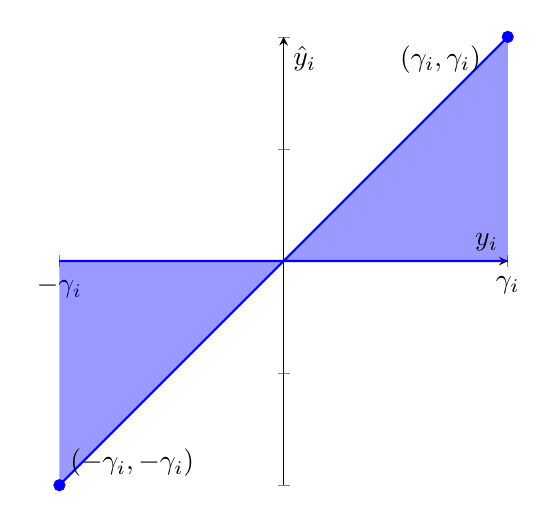
\begin{tikzpicture}
		\begin{axis}[
			xlabel={$y_i$},
			ylabel={$\hat{y}_i$},
			xmin=-2, xmax=2,
			ymin=-2, ymax=2,
			axis lines=center,
			samples=100, 
			unit vector ratio=1 1 1, scale=1, xtick   = {-2,2},
			xticklabels = {$-\gamma_i$,$\gamma_i$},
			yticklabels = {},
			]
			\addplot[blue, thick, fill=blue, fill opacity=0.4] {x} \closedcycle; 
			\addplot[blue, thick] {0}; 
			
			\addplot[only marks, mark=*, mark size=2pt, blue] coordinates {(-2,-2)};
			\node[label={above:$(-\gamma_i,-\gamma_i)$}] at (axis cs: -1.35, -2.1) {};
			
			\addplot[only marks, mark=*, mark size=2pt, blue] coordinates {(2,2)};
			\node[label={above:$(\gamma_i,\gamma_i)$}] at (axis cs: 1.4, 1.5) {};
		\end{axis}
	\end{tikzpicture}
	
   Based on above constraints, we can sketch this simplified model:
\begin{enumerate}
	\item For each input node, each output node, and each pre-activation and post-activation node in the hidden layers,  set one variable $y_i$. 
	\item Set constraints for input nodes.
	\item Set linear constraints . In this case, since the meaning of $y_i$ is $x_i-x'_i$, this constraints will not use the bias.
	\item Between pre- and post- activation nodes, set the MILP constraint described above.
\end{enumerate}
	
	The key point is that, although this model sets 3 variables (and their binary variables) for each node in the network, only $y_i$  contributes to the final results, and we can ignore $x_i,x_i'$ (and their binary variables) during the optimization.
	
	As a result, we can relax the binary variables used to $\hat{x}_i = \ReLU(x_i)$ and $\hat{x}'_i = \ReLU(x'_i)$.
	
	Now the simplified model contains the same number of binary variables as the MILP model for local robustness. Hence this model runs much faster compared to the previous one. The trade-off is lower accuracy compared to the first model under unlimited time. In practice, with a reasonable timeout, this simplified model can usually obtain a better bound.
	
	One major disadvantage of this model is that the solution obtained through optimization may not be valid-i.e., the output computed by the network on the optimized inputs may not equal the output value in the solution. Nevertheless, it is meaningful to compute the upper bound. 
	
%	However, in practice, with a reasonable timeout, this simplified model can usually obtain a better bound.
%	
	\subsection{Improving the Accuracy of the Simplified Model}
	We can remove the disadvantage and improve the accuracy of the above simplified model by modifying the constraints, at the cost of increased computational time — a trade-off between accuracy and speed. 
	
%	(This model has the same binary set, although the meaning of binary variable for $y_i$ is somehow different.)
	
	
	
%	The exact constraints for $$ \begin{align*}
%		&\hat{y}_i \geq -\hat{x}'_i \hspace*{1ex} \wedge \hspace*{1ex} \hat{y}_i \leq -\hat{x}'_i+a\beta_i  \hspace*{1ex}\wedge\hspace*{1ex} x_i'+y_i \leq a\beta_i \hspace*{1ex}\wedge\hspace*{1ex}  x_i'+y_i \geq (1-a)\alpha_i \\
%		&\hat{y}_i \geq -\hat{x}'_i+(x_i'+y_i) \hspace*{1ex}\wedge\hspace*{1ex} \hat{y}_i \leq -\hat{x}'_i+(x_i'+y_i) +(a-1)\alpha_i \\
%	\end{align*} 
%	
%	
%	Moreover, we can add two more natural constraints: $x_i'+y_i \geq \alpha_i \hspace*{1ex}\wedge\hspace*{1ex}  x_i'+y_i \leq \beta_i.$
	
	
	
	Given $\gamma_i$ as the upper bound of $y_i$, $\alpha_i,\beta_i$ be the upper and lower bound of $x_i,x_i'$, 
	the precise  constraints for $\hat{y}_i = \ReLU(x'_i+y_i)-\ReLU(x'_i)$ (along with $\hat{x}'_i=\ReLU(x'_i)$) are as follows:
	\begin{align*}
		& \begin{aligned}
			y_i + x'_i &\leq a\beta_i        &\quad\quad
			y_i + x'_i &\geq (1-a)\alpha_i \\
			x'_i       &\leq a'\beta_i       & 
			x'_i       &\geq (1-a')\alpha_i \\
			\hat{y}_i  &\leq a\gamma_i       &
			\hat{y}_i  &\geq -a'\gamma_i \\
			\hat{y}_i  &\leq y_i + (1-a)\gamma_i  &
			\hat{y}_i  &\geq y_i - (1-a')\gamma_i \\
			\hat{y}_i  &\leq -x'_i + a\beta_i &
			\hat{y}_i  &\geq -x'_i + (1-a')\alpha_i \\
			\hat{y}_i  &\leq y_i + x'_i + (1-a)(-\alpha_i) &
			\hat{y}_i  &\geq y_i + x'_i + a'(-\beta_i)
		\end{aligned}
	\end{align*} Here, $a,a'$ are binary variables, and $a'$ is also the binary variable in the constraints for $\hat{x}'_i=\ReLU(x'_i)$. 
	
	Similar to the second model, the constraints on $x_i$ for $\hat{x}_i=\ReLU(x_i)$ are not necessary, or at least can be relaxed without any loss in accuracy.
	
%	\begin{align*}
%		& y_i+x'_i \leq a\beta_i \quad\wedge \quad y_i+x'_i\geq (1-a)\alpha_i\\	
%		& x_i' \leq a'\beta_i \quad\wedge \quad x_i'\geq (1-a')\alpha_i\\
%		&\hat{y}_i \leq a\gamma_i \quad\wedge \quad	\hat{y}_i \geq -a'\gamma_i \\
%		&	\hat{y}_i \leq y_i+(1-a)\gamma_i \quad\wedge \quad	\hat{y}_i \geq y_i - (1-a')\gamma_i \\
%		&	\hat{y}_i \leq -x'_i+a\beta_i \quad\wedge \quad	\hat{y}_i \geq -x'_i+(1-a')\alpha_i \\
%		&	\hat{y}_i \leq y_i+x'_i+(1-a)(-\alpha_i)\quad\wedge \quad	\hat{y}_i \geq y_i+x'_i+a'(-\beta_i) \\
%	\end{align*} 
	
	The following plot illustrates the constraints described above.
	
	\hspace*{-10ex}
	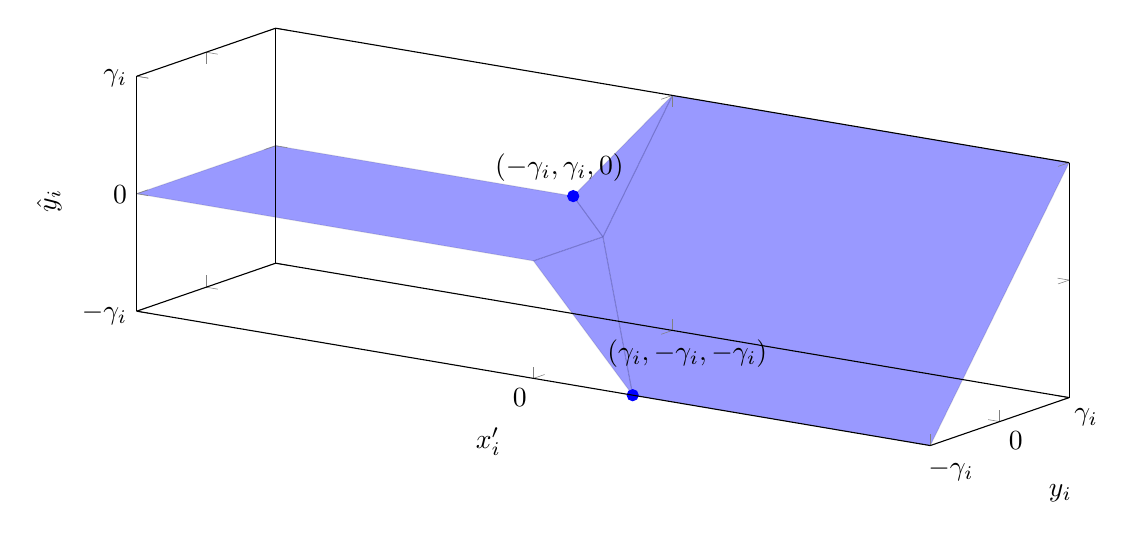
\begin{tikzpicture}
		\begin{axis}[	axis on top, xlabel = \(x'_i\),
			ylabel = {\(y_i\)}, zlabel = \(\hat{y}_i\),
			set layers=default,
			xmax = 4, xmin = -4,
			ymax = 1, ymin = -1,		
			zmax = 1, zmin = -1,
			unit vector ratio=1 1 1, scale=2.5,  ytick   = {-1,0,1},
			yticklabels = {$-\gamma_i$,$0$,$\gamma_i$}, xtick = {0},
			xticklabels = {$0$}, ztick   = {-1,0,1},
			zticklabels = {$-\gamma_i$,$0$,$\gamma_i$},
			view={35}{14},
			]
			\addplot3[ fill=blue,opacity=0.1, fill opacity=0.4] 
			coordinates {
				(0,0,0) (-1,1,0) (-4,1,0) (-4,-1,0) (0,-1,0) (0,0,0)
			};
			
			\addplot3[	fill=blue,opacity=0.1, fill opacity=0.4] 
			coordinates { (0,0,0) (0,1,1) (4, 1, 1) (4, -1, -1) (1,-1,-1) (0,0,0)
			};
			
			\addplot3[	fill=blue,opacity=0.1, fill opacity=0.4	] 
			coordinates { (0,0,0)  (-1,1,0) (0,1,1) (0,0,0)
			};
			
			\addplot3[	fill=blue,opacity=0.1, fill opacity=0.4	] 
			coordinates { (0,0,0)  (0,-1,0) (1,-1,-1) (0,0,0)
			};
			
			\addplot3[only marks, mark=*, mark size=2pt, blue] coordinates {(1,-1,-1)};
			\node[label={$(\gamma_i,-\gamma_i, -\gamma_i)$}] at (axis cs: 1.2, -0.5 ,-1) {};
			
			\addplot3[only marks, mark=*, mark size=2pt, blue] coordinates {(-1,1,0)};
			\node[label={$(-\gamma_i,\gamma_i, 0)$}] at (axis cs: -1, 0.8 ,0) {};			
			
		\end{axis}
	\end{tikzpicture}
	
	In practice, when we relax the constraints for a node, we will convert $a_i$ and $a_i'$ to continuous variables together. In principle, we can also choose to change  only one of those two binary variables.
	
%	The relaxation of this model is similar: let $a$s and $a'$s be continuous variables instead of binary/integer variables. Unlike the first model in this section, relaxing a few nodes does not lose too much accuracy.
	
	A special relaxation approach of this model is to treat the binary variables $a'$ appearing in the above constraints and the binary variables for $\hat{x}'_i=\ReLU(x'_i)$ as distinct variables, and relax only the latter. 
	
	This approach has a similar disadvantage as the model in the previous section: the output computed by the network on the optimized inputs may not equal the output value in the solution. Similarly, it is meaningful to compute the upper bound using this approach. 
	
	
	\section{Experimental Evaluation}
	
	We implemented our code in Python 3.8.
	Gurobi 9.52 was used for solving LP and MILP problems. We conducted our evaluation on an AMD Threadripper 7970X  ($32$ cores$@4.0$GHz) with 256 GB of main memory and 2 NVIDIA RTX 4090. 
	
	We will do experiments on two networks for MNIST dataset and another physical model. Two MNIST have the same structure. They are full-connected DNN with 5, 10 outputs and 784 inputs; each hidden layer has 100 neurons. One of them is a normally trained neural network and another is for trained for adversarial robustness. We call them MNIST $5\times100$-Normal and MNIST $5\times 100$-DiffAI. As the name shows MNIST $5\times 100$-DiffAI has a better robustness. The physical network is a simplified model with 10 input neurons, 26 output neurons, and 2 hidden layers with 50 neurons each.
	
	\subsection{Comparison of different modelings}
	
	\subsection{Comparison of different scoring algorithms}
	
	\section{Conclusion}
	
	TODO
	
	
	\bibliography{references}
	\bibliographystyle{plain}
	
	
	\bigskip
	
	\appendix
	
	
	
\end{document}


